\documentclass[11pt,letterpaper]{article}
\usepackage[T1]{fontenc}
\usepackage[utf8]{inputenc}
\usepackage{lmodern,microtype}
\usepackage[margin=0.78in,top=0.7in,bottom=0.7in]{geometry}
\usepackage{xcolor,booktabs,array,longtable,tabularx,enumitem}
\usepackage{tikz}
\usetikzlibrary{arrows.meta,positioning}
\usepackage{hyperref,xurl,fancyhdr}
\definecolor{ink}{HTML}{19364A}
\hypersetup{colorlinks=true,urlcolor=ink,linkcolor=ink,pdftitle={Resonant OS SDK Final Engineering and Verification Report},pdfauthor={Resonant OS SDK Engineering}}
\setlength{\parindent}{0pt}
\setlength{\parskip}{6pt}
\setlength{\emergencystretch}{2em}
\renewcommand{\arraystretch}{1.18}
\pagestyle{fancy}\fancyhf{}
\fancyfoot[L]{\scriptsize SDK-DEMO-003R \quad Final engineering and verification report}
\fancyfoot[R]{\scriptsize\thepage}
\renewcommand{\headrulewidth}{0pt}\renewcommand{\footrulewidth}{0pt}
\newcommand{\reportsection}[1]{\phantomsection\addcontentsline{toc}{section}{#1}{\Large\bfseries\color{ink}#1}\par\vspace{5pt}}
\begin{document}
\thispagestyle{empty}
\vspace*{1.1in}
{\large RESONANT OS SDK\par}
\vspace{0.3in}
{\Huge\bfseries Final Engineering\\[7pt]and Verification Report\par}
\vspace{0.25in}
{\Large SDK-DEMO-003R\par}
\vspace{0.6in}
{\large T1 through T7 and T7.1\par}
\vspace{0.65in}
\begin{tabular}{@{}ll}
Prepared for & Tom, technical reviewer and SDK collaborator\\[8pt]
Report date & 28 September 2026\\[8pt]
Disposition & Review and acceptance work complete\\[8pt]
Verification & Independent exact-SHA PASS, issue \#51\\[8pt]
Version & Final report 1.0
\end{tabular}
\vspace{0.4in}\par
Final accepted candidate\par
{\small\ttfamily 180f3067906d4782df5b923ca46ef77b80828333}\par
\vfill
Scope: Resonant OS SDK corrections, architectural boundaries, regression coverage and final independent acceptance. Future hardening is recorded separately.

\clearpage
\reportsection{Executive summary}
Tom, your SDK review findings have been worked through from T1 through T7, including the T6.1 credential audit and T7.1 graphical-test correction. SDK-DEMO-003R review and acceptance work is complete for candidate 180f3067906d4782df5b923ca46ef77b80828333. Independent exact-SHA verification in work-order issue \#51 reports PASS with no source mutation. [E51]\par
The corrections establish clearer ownership of authority across the Resonant OS SDK. Requests identify an add-on and an intended action; the host resolves privileged credentials and administrative destinations. Discovery reports state without installing. Explicit install creates denied registry state, and explicit grant or revoke coordinates that authoritative state with the upstream enforcement projection.\par
The work also improved integration contracts and the operator experience. Missing install handlers fail at service construction. The browser displays host state, exposes install, grant and revoke as explicit actions, suppresses duplicate pending actions, and re-reads authority after mutations. Generic credential provisioning replaces per-demo wiring while retaining separate scoped-bearer and privileged-admin credential classes.\par
Real browser and extension testing found defects that narrower tests missed: stale admin-revoke request bodies and malformed host-owned endpoint URLs, a certification environment running OpenCode 1.14.33 instead of the required 1.18.4, and a graphical assertion that could observe unrelated card text before grant completion. T7 additionally closed a fail-open upstream restart default and the missing grant-to-upstream convergence path.\par
Final independent results include Browser-first 2259 passed out of 2260, exit 0, no failures and one macOS-only test skipped on Linux; real graphical Extension 5/5; Browser-host 13/13; Security/adversarial 12/12; T2 focused gates 6/6 and 2/2; and artifact verification PASS. Unit/Vitest and SDK stages also passed. These results are scoped acceptance evidence, not a claim of universal security or production completeness.\par
Future hardening remains separate: a host-mediated proxy, credential expiry and rotation, encrypted storage, credential-file permission checks, finer operator consent, reconciliation tooling, reinstall semantics, and better documentation and finding-to-test traceability. None is being represented as an unresolved blocker to the accepted SDK-DEMO-003R work.\par
One reporting correction matters: the T7.1 record attributes the loose /granted/i match to ``Grant requested capabilities.'' That literal does not match. Source inspection identifies installation.grantedCapabilities in the card's explanatory text as a valid premature match. The synchronization defect, exact-label correction and independent final PASS remain supported. Section 7 records the distinction transparently.\par
\clearpage
\reportsection{Contents and review disposition}
{\small\begin{longtable}{@{}>{\raggedright\arraybackslash}p{0.630in}@{\hspace{0.16in}}>{\raggedright\arraybackslash}p{5.359in}@{\hspace{0.16in}}>{\raggedright\arraybackslash}p{0.630in}@{}}\toprule
\textbf{Section} & \textbf{Topic} & \textbf{Page}\\\midrule\endhead
1 & Host authority and read-only discovery & 4\\
2 & Install contract and live integration findings & 5\\
3 & Revocation convergence & 6\\
4 & Operator lifecycle & 7\\
5 & Generic credentials and boundary hardening & 8\\
6 & Endpoint enforcement & 9\\
7 & Graphical integration closure & 10\\
8 & Final SDK authority model & 11\\
9 & Verification methodology and lineage & 12\\
10 & Final acceptance & 13\\
11 & Recommended future hardening & 14\\
A & Exact commit lineage and evidence register & 15\\
B & Finding-to-test and source traceability & 16\\
C & Audit qualifications and report provenance & 17\\
\bottomrule\end{longtable}}
\vspace{3pt}{\normalsize\bfseries Review item matrix}\par
{\small\begin{longtable}{@{}>{\raggedright\arraybackslash}p{0.630in}@{\hspace{0.16in}}>{\raggedright\arraybackslash}p{5.149in}@{\hspace{0.16in}}>{\raggedright\arraybackslash}p{0.841in}@{}}\toprule
\textbf{Item} & \textbf{Accepted correction} & \textbf{Status}\\\midrule\endhead
T1 & Host-owned administrative authority & CLOSED\\
T2 & Status and discovery do not install & CLOSED\\
T3 & Required install handler and integration closure & CLOSED\\
T4 & Registry and upstream revocation converge & CLOSED\\
T5 & Explicit operator install, grant and revoke UI & CLOSED\\
T6 & Generic host-owned credential provisioning & CLOSED\\
T6.1 & Credential source and boundary hardening & CLOSED\\
T7 & Closed startup and symmetric endpoint convergence & CLOSED\\
T7.1 & Authoritative graphical-test synchronization & CLOSED\\
\bottomrule\end{longtable}}
Closure refers to the accepted review scope at the final candidate, supported by the lineage and independent verification below. Deferred deployment and architecture work is listed separately.\par
\clearpage
\reportsection{1  Host authority and read-only discovery}
\vspace{3pt}{\normalsize\bfseries T1  Host-owned administrative authority}\par
Original finding. Administrative revoke accepted caller-controlled upstreamAdminUrl and adminToken. This allowed request data to determine privileged outbound authority. Investigation traced the request through the workspace host handler to the upstream administrative fetch. [S1]\par
{\small\ttfamily\raggedright REQUEST DESCRIBES INTENT.\\HOST DETERMINES AUTHORITY.\par}
Correction. The caller identifies the add-on and requested action. The host resolves the administrative destination and credential from host provisioning, keyed by add-on identity. The admin-revoke handler rejects any supplied upstreamAdminUrl or adminToken field with permission-denied before contacting the upstream. Missing host configuration denies the operation. The follow-up validation rejects null, arrays and other malformed request shapes as invalid-event instead of throwing a native destructuring error.\par
Verification. Commits c54bbee5 and 5ee4dfd1 establish the boundary and malformed-input hardening. The adversarial suite covers caller injection, unconfigured add-ons and malformed requests; host-service regressions preserve required route wiring. The accepted cumulative T1--T3/live candidate is c869a928, independently passed in \#28 after environment qualification. Status: CLOSED. [E28, S1, S4]\par
\vspace{3pt}{\normalsize\bfseries T2  Discovery reports state without installation}\par
Original finding. executeAddonsStatus installed discovered manifests. Earlier re-poll protection reduced grant wiping but still made a status request an installation action. Investigation separated discovery projection, canonical manifest caching and registry mutation. [S1, S5]\par
{\small\ttfamily\raggedright READ/DISCOVERY REPORTS STATE.\\EXPLICIT INSTALL MUTATES STATE.\par}
Correction. Status now caches full canonical manifests for subsequent installation and projects installed/granted state from registry snapshots. It does not invoke registry.install, grant or revoke. Explicit installation is separate and grants nothing; requested capabilities begin denied. Existing grants survive status polling.\par
Verification. Six read-only tests cover initial discovery, repeated polling, explicit installation, duplicate prevention, discovery failure and registry-grant reporting. Two grant-regression tests protect grants across polling. T2-5 was strengthened to inject an actual discovery exception and assert discovery-failed, an empty result and unchanged empty registry state. Final independent results are 6/6 and 2/2. Status: CLOSED. [E51, S5]\par
Scope precision. Bootstrap retains a separate compatibility path that may register a cached, absent manifest with denied grants. T2 establishes read-only status/discovery; it does not establish that every route classified as ``read'' is free of registration side effects. Bootstrap never creates granted authority. [S1]\par
\clearpage
\reportsection{2  Install contract and live integration findings}
\vspace{3pt}{\normalsize\bfseries T3  Required host contract}\par
Making executeWorkspaceAddonInstall a required host-service handler exposed stale service constructions. The correction retained that contract: service construction fails fast when the handler is absent, and the install route remains wired with addon-runtime-control. T1-related fixture updates supplied the workspace handlers; T3 commit 4e7a144c added an explicit missing-install-handler regression. This is contract and integration closure, not a new security architecture. Status: CLOSED. [S2, S6]\par
\vspace{3pt}{\normalsize\bfseries Admin-revoke HTTP 500 in the graphical path}\par
Real extension tests failed for both Counter and SDK Guide with 500 rather than the expected 200. The investigation identified two distinct defects. First, both test clients still sent pre-T1 privileged URL/token fields. T1 correctly rejected those fields, but the then-current transport error mapping surfaced the rejection as HTTP 500. Second, the host mapping itself contained invalid Echo/Counter URLs with uninterpolated \$\{...\} strings and an incorrect SDK Guide port of 3403. [E25, S7]\par
Commit c869a928 changed the live test bodies to intent-only \{ addonId, granted \} and corrected the host-owned destinations to the manifest-aligned loopback ports 47321, 47322 and 47323. It did not relax the injection guard. A new live-bridge regression exercised successful host mapping and injection denial; the engineering record reports that it failed before the correction and passed afterward. Both graphical lifecycle paths then passed, with the extension suite reaching 4/4. [E25]\par
The HTTP error-family improvement was completed separately: T4 gave revoke/admin-revoke the harness transport boundary, and T5 aligned install/grant. The final routes distinguish policy 4xx from runtime 5xx failures. T6 subsequently replaced the temporary literal per-demo destinations with generic provisioning. This chronology avoids attributing all later hardening to the HTTP 500 fix. [S2, S3]\par
\vspace{3pt}{\normalsize\bfseries OpenCode environment qualification}\par
The certification environment resolved OpenCode 1.14.33 while browser-first/host/opencode-version.json required 1.18.4. This was an environment mismatch, not an SDK architecture defect. The environment qualification record reports upgrading the existing arm64 installation to exactly 1.18.4, verifying the SDK's trusted-root resolution and the version-pin scenario, and leaving SDK source and its expected version unchanged. [E27, S8]\par
The first c869a928 verification still exposed the mismatch. The fresh independent \#28 run on the same SHA passed after qualification: Browser-first 2213/2214 and Extension 4/4. The single excluded test was the platform-specific macOS sandbox test. Narrow green tests were therefore insufficient until the real path and its environment were qualified. [E28]\par
\clearpage
\reportsection{3  Revocation convergence}
\vspace{3pt}{\normalsize\bfseries T4  One authority and its enforcement projection}\par
Original finding. Registry revoke and the upstream administrative deny channel could change independently. A denied registry could coexist with an upstream still accepting a previously issued bearer, while upstream denial alone could leave registry state reporting grants. [S1, S9]\par
{\small\ttfamily\raggedright Registry grant state = authoritative source of truth\\Upstream enforcement = projection of that authority\par}
Correction. Both operator revoke surfaces converge registry grants and upstream enforcement. The shared convergence helper computes the target grant surface and coordinates the writes. Administrative revoke can deny the whole surface or perform the supported explicit regrant. Partial capability revoke preserves the other registry entries; the current upstream gate remains open while any capability is granted.\par
{\small\begin{longtable}{@{}>{\raggedright\arraybackslash}p{0.841in}@{\hspace{0.16in}}>{\raggedright\arraybackslash}p{2.207in}@{\hspace{0.16in}}>{\raggedright\arraybackslash}p{3.573in}@{}}\toprule
\textbf{Transition} & \textbf{Order} & \textbf{Failure interpretation}\\\midrule\endhead
DENY & 1. Close upstream\newline 2. Persist registry denial & If denial persistence fails after upstream closure, enforcement stays closed and the operation reports failure.\\
ALLOW & 1. Persist registry grant\newline 2. Open upstream & If upstream opening fails from a closed state, the registry may show a grant while enforcement stays closed; the operation reports failure.\\
\bottomrule\end{longtable}}
This is not a distributed transaction. A successful return means both writes completed. Revision checks surface conflicting registry updates, and reapplying the same desired state supports retry. There is no claim of atomic cross-process commit or automatic recovery from every partial failure.\par
Failure boundary. The ordering avoids prematurely opening authority. It cannot guarantee remote closure if the initial upstream-close request itself fails against an already-open service; that revoke fails and must be retried. Likewise, lost acknowledgments cannot be equated with confirmed remote state. These distinctions are necessary when interpreting ``fail closed.'' [S1, S9]\par
\vspace{3pt}{\normalsize\bfseries Bootstrap and regression protection}\par
Bootstrap derives token delivery from registry grants rather than manifest presets. Existing denied installations stay denied. If an installation is absent but a canonical manifest is cached, bootstrap may register it with denied grants; it does not restore prior grants or open enforcement. The regression tests cover this even after registry removal. [S1, S9]\par
Seven T4 tests cover both revoke channels, supported administrative regrant, bootstrap non-resurrection, privileged-field injection, upstream failure and retry/idempotence. Independent \#39 passed c57d4d0f, including Browser-first 2220/2221 and graphical Extension 4/4. Status: CLOSED. T7 later completed ordinary /grant convergence and restart-safe upstream defaults; those were not already solved by T4. [E39]\par
\clearpage
\reportsection{4  Operator lifecycle}
\vspace{3pt}{\normalsize\bfseries T5  Explicit actions and authoritative state}\par
{\small\ttfamily\raggedright Discover -> Install -> Denied -> Grant -> Granted\\Granted -> Revoke -> Denied\par}
The Add-ons card exposes explicit operator installation, grant and revoke. Discovery alone offers installation and reports no granted authority. Install registers the add-on with denied capabilities. Grant requests currently outstanding capabilities; revoke requests withdrawal of the currently granted capabilities. [S10]\par
The browser does not invent authority. The displayed status and capability chips derive from the host registry projection returned by /addons/status. Manifest grant presets describe approvable requests; they are not current authority. The request shape preserves the declared capability scope and revocation behavior.\par
The operator UI installs with \{ addonId \}. The host resolves the canonical manifest from its discovery cache. The browser does not send an administrative URL or token, and it does not call upstream /admin routes directly. The service also retains a \{ manifest \} argument for existing host-side uses; the accepted change should not be overstated as a universal public payload allowlist. [S1, S2, S10]\par
{\small\begin{longtable}{@{}>{\raggedright\arraybackslash}p{1.507in}@{\hspace{0.16in}}>{\raggedright\arraybackslash}p{5.273in}@{}}\toprule
\textbf{Condition} & \textbf{Operator behavior}\\\midrule\endhead
Mutation pending & Disable the add-on's action buttons and suppress duplicate requests.\\
Mutation succeeds & Re-read /addons/status; show the host result rather than optimistically changing local authority.\\
Policy rejection & Show a 4xx policy error and re-read the host state.\\
Runtime or network failure & Show a failure or connection guidance and re-read when possible; do not report the action as successful.\\
\bottomrule\end{longtable}}
State and action outcome are distinct. A partial grant failure can leave a persisted registry grant while upstream opening failed. An authoritative refresh may therefore show that grant together with a failure message; it must not be read as confirmation that enforcement has opened. Operator-visible reconciliation remains useful future work. [S1, S10]\par
\vspace{3pt}{\normalsize\bfseries Verification and graphical proof}\par
Nine UI regressions cover discovered and denied state, grant/revoke refresh, policy/runtime errors, pending duplicate suppression, read-only refresh and absence of privileged fields. Five bridge tests cover installation state, canonical addonId resolution, unknown IDs and transport/error boundaries. [S11]\par
The real extension test exercises Install  ->  Grant  ->  bearer HTTP 200  ->  Revoke  ->  the same bearer HTTP 403. Independent \#41 accepted 20726e39 with Extension 5/5 and Browser-first 2234/2235. T7.1 later tightened the test's synchronization without changing this lifecycle or weakening enforcement. Status: CLOSED. [E41, E51, S12]\par
\clearpage
\reportsection{5  Generic credentials and boundary hardening}
\vspace{3pt}{\normalsize\bfseries T6  Provision by identity and purpose}\par
Earlier provisioning required per-demo token maps, literal administrative endpoints and bespoke flags/environment variables. Each new add-on required launcher changes. T6 replaced this wiring with workspace-addon-credentials.mjs, a host-owned resolver accepting add-on identity, credential purpose and, for endpoint derivation, the host's canonical manifest entrypoint. [S3]\par
{\small\begin{longtable}{@{}>{\raggedright\arraybackslash}p{1.156in}@{\hspace{0.16in}}>{\raggedright\arraybackslash}p{2.364in}@{\hspace{0.16in}}>{\raggedright\arraybackslash}p{3.100in}@{}}\toprule
\textbf{Class} & \textbf{Returned material} & \textbf{Permitted boundary}\\\midrule\endhead
Scoped bearer & Add-on identity, purpose and token & May cross the sandbox/bootstrap boundary for host-granted capabilities.\\
Privileged admin & Add-on identity, purpose, administrative URL and token & Trusted host/admin channel only; never iframe, status or bootstrap.\\
\bottomrule\end{longtable}}
Generic provisioning is not one undifferentiated bag of secrets. The resolver returns only the selected credential class. The operator-started upstream receives its own bearer and admin verification material; ``host-only'' excludes browser/add-on UI delivery, not the trusted upstream that validates the administrative call. Provisioning is config/environment-backed, loaded at startup into process memory, and rotation is restart-bound. No encrypted vault, per-grant minting or expiry is implemented.\par
\vspace{3pt}{\normalsize\bfseries T6.1  Audit corrections}\par
The audit found raw credential JSON accepted through process argv, acceptance of 0.0.0.0 as an administrative destination, and wording that overstated resolver authentication. The raw-secret JSON flag is no longer read; a credential-file path is allowed. Source precedence is CLI file reference, environment file path, environment JSON, then an empty fail-closed configuration. The old raw flag alone provides no credentials. [S3, S13]\par
The documented destination policy is true loopback: 127.0.0.0/8, ::1 and localhost; 0.0.0.0 is rejected, as are tested external destinations and non-HTTP(S) schemes. The resolver is explicitly an internal lookup, not an authentication boundary. Trusted host call sites bind the requested identity to registry/install state and obtain endpoint context from the host-owned manifest cache before resolving credentials.\par
{\small\ttfamily\raggedright Trusted host caller -> authoritative add-on identity\\                    -> credential resolver\par}
Verification. Sixteen credential tests cover purpose separation, distinct add-ons, absent/invalid material, secret-free errors, provisioning precedence, raw-argv removal, bind-any rejection, accepted loopback cases, bootstrap bearer-only delivery and credential-free status. The audit documented production call sites. The initial T6 SHA 30197261 is superseded by b8735970, independently passed in \#45. T6 and T6.1: CLOSED. [E45, S13]\par
\clearpage
\reportsection{6  Endpoint enforcement}
\vspace{3pt}{\normalsize\bfseries T7  Close the startup and grant-direction gaps}\par
Investigation found that Echo, Counter and SDK Guide initialized hostGranted = true. A restarted upstream therefore reopened mutating endpoints despite revoked registry authority, allowing a stale but valid bearer to become effective again. Ordinary /addons/workspace/grant changed the registry without opening upstream enforcement; revoke converged both layers, but ordinary regrant did not. [S1, S14]\par
T7 changed all three fresh upstream defaults to hostGranted = false and made ordinary grant converge through the host-owned administrative channel. It also rejected 0.0.0.0 discovery entrypoints, aligning the discovery case with the T6.1 bind-any restriction. The correction closed the demonstrated gap without implementing the deferred host-mediated proxy.\par
{\small\begin{longtable}{@{}>{\raggedright\arraybackslash}p{1.261in}@{\hspace{0.16in}}>{\raggedright\arraybackslash}p{4.046in}@{\hspace{0.16in}}>{\raggedright\arraybackslash}p{1.313in}@{}}\toprule
\textbf{Lifecycle event} & \textbf{Authoritative action and enforcement} & \textbf{Bearer result}\\\midrule\endhead
Fresh upstream & Starts hostGranted = false & 403\\
Explicit grant & Persist registry authority, then open upstream & 200\\
Explicit revoke & Close upstream, then persist registry denial & 403\\
Restart after revoke & Fresh process starts closed & 403 for stale bearer\\
Explicit regrant & Persist grant, then reopen upstream & 200\\
\bottomrule\end{longtable}}
These results concern a valid configured bearer on the protected mutating API. Missing or incorrect authentication is a separate condition, typically 401; no configured bearer can produce 503. The in-memory gate is currently add-on-wide, based on whether any capability remains granted, rather than a general per-operation capability evaluator.\par
\vspace{3pt}{\normalsize\bfseries Endpoint and route verification}\par
Eight endpoint regressions cover fresh denial across all three servers, grant success, converged revoke, stale-bearer denial after restart, regrant, unavailable-upstream failure, forged grant fields and bind-any discovery rejection. The route completeness audit inspects declared route metadata in both directions: every workspace route must be classified, and every classified route must exist. [S14, S15]\par
Install, grant, revoke and admin-revoke require addon-runtime-control, loopbackHostOnly and harness error mapping. Grants lookup and bootstrap require addon-runtime-read. A new unclassified /addons/workspace/* route fails the audit. Bootstrap's read classification does not remove its denied-registration compatibility behavior described in Section 1.\par
Candidate f99667b4 passed the independent Browser-first stage but failed the graphical Extension stage; it was not accepted. Final closure uses corrected candidate 180f3067 and \#51. T7 production enforcement is identical between those two candidates. Status: CLOSED at the final candidate. [E49, E51]\par
\clearpage
\reportsection{7  Graphical integration closure}
\vspace{3pt}{\normalsize\bfseries T7.1  The failed candidate remains part of the record}\par
Independent \#49 tested f99667b4641a51861d65a4fad8e4bd7aa07e7e06 without source mutation. Browser-first passed 2259/2260, but Extension passed four of five tests and failed overall. The failing test was ``T5 real extension exercises operator grant/revoke UI (install -> grant -> revoke),'' with 403 !== 200. It was one failed test, not four failures. [E49]\par
The engineering investigation recorded that the card remained DENIED with a mutation pending when the whole-card wait returned. The subsequent bearer request could reach the upstream before grant convergence and correctly receive 403. The report records 9/12 full-suite failures before correction, passage in isolation, and 0/12 full-suite failures afterward. Those reproduction counts are engineering evidence; independent acceptance comes from \#51. [E50]\par
\vspace{3pt}{\normalsize\bfseries Mechanically corrected explanation}\par
The old helper polled card.innerText() with /granted/i. Both the work-order narrative and the committed findings incorrectly say this matched ``Grant requested capabilities.'' A direct JavaScript check shows that it does not. The actual card includes explanatory text mentioning installation.grantedCapabilities, which does match /granted/i regardless of the header's authority status. The source therefore supports the premature whole-card match and race, but not the stated button-label attribution. [S10, S12, S16]\par
{\small\ttfamily\raggedright /granted/i.test("Grant requested capabilities")  // false\\/granted/i.test("installation.grantedCapabilities") // true\par}
\vspace{3pt}{\normalsize\bfseries Correction and acceptance}\par
T7.1 restricts the wait to the dedicated .addon-card-header span and compares its trimmed value case-insensitively with the exact expected state: Discovered, Denied or Granted. The bearer request is issued only after the authoritative label reaches Granted, following the UI's completed mutation and re-read. It no longer treats arbitrary card prose as a completion signal.\par
{\small\ttfamily\raggedright text.trim().toLowerCase() === label.toLowerCase()\par}
The final diff changes only the graphical test and SDK-DEMO-003-FINDINGS.md. It makes no production-source change and does not weaken the fail-closed endpoint. Existing endpoint tests separately assert registry grant, upstream gate state and HTTP result; the graphical test verifies the real operator sequence.\par
Independent \#51 then passed the corrected exact SHA with Extension 5/5 and all cumulative gates green. The rejected T7 candidate is retained in the lineage because it demonstrates why engineering PASS and isolated success were not sufficient acceptance evidence. Status: CLOSED. [E51]\par
\clearpage
\reportsection{8  Final SDK authority model}
\begin{center}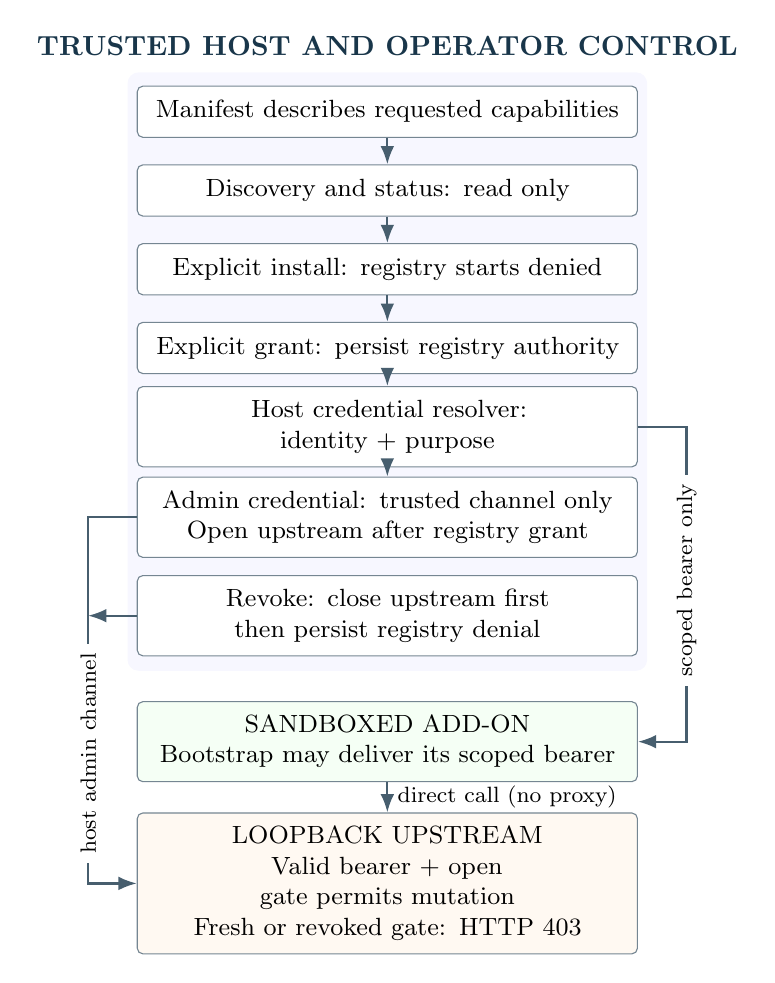
\begin{tikzpicture}[x=1cm,y=1cm,>=Latex,
font=\fontsize{9}{11}\selectfont,
box/.style={draw=ink!60,rounded corners=2pt,align=center,fill=white,minimum height=.65cm,text width=6cm,inner sep=5pt},
arr/.style={->,thick,draw=ink!80}]
\fill[blue!3,rounded corners] (-3.3,-.45) rectangle (3.3,-8.05);
\node[font=\fontsize{10}{12}\selectfont\bfseries,text=ink] at (0,-.12) {TRUSTED HOST AND OPERATOR CONTROL};
\node[box] (m) at (0,-.95) {Manifest describes requested capabilities};
\node[box] (d) at (0,-1.95) {Discovery and status: read only};
\node[box] (i) at (0,-2.95) {Explicit install: registry starts denied};
\node[box] (g) at (0,-3.95) {Explicit grant: persist registry authority};
\node[box] (r) at (0,-4.95) {Host credential resolver: identity + purpose};
\node[box] (a) at (0,-6.10) {Admin credential: trusted channel only\\Open upstream after registry grant};
\node[box] (v) at (0,-7.35) {Revoke: close upstream first\\then persist registry denial};
\draw[arr] (m)--(d);\draw[arr] (d)--(i);\draw[arr] (i)--(g);\draw[arr] (g)--(r);\draw[arr] (r)--(a);
\node[box,fill=green!4] (s) at (0,-8.95) {SANDBOXED ADD-ON\\Bootstrap may deliver its scoped bearer};
\node[box,fill=orange!5] (u) at (0,-10.75) {LOOPBACK UPSTREAM\\Valid bearer + open gate permits mutation\\Fresh or revoked gate: HTTP 403};
\draw[arr] (r.east) -- (3.8,-4.95) -- (3.8,-8.95) -- (s.east);
\node[rotate=90,fill=white,font=\fontsize{8}{9}\selectfont] at (3.8,-6.9) {scoped bearer only};
\draw[arr] (a.west) -- (-3.8,-6.1) -- (-3.8,-10.75) -- (u.west);
\draw[arr] (v.west) -- (-3.8,-7.35);
\node[rotate=90,fill=white,font=\fontsize{8}{9}\selectfont] at (-3.8,-9.1) {host admin channel};
\draw[arr] (s)--node[right,font=\fontsize{8}{9}\selectfont,align=left]{direct call (no proxy)}(u);
\end{tikzpicture}\end{center}
The manifest describes requested capabilities. Discovery caches canonical definitions and projects state. Explicit installation creates denied registry entries; explicit host grant persists authority before opening the upstream. Revocation closes upstream enforcement before persisting denial. Bootstrap delivers only scoped bearer material for granted capabilities. [S1--S3, S10, S14]\par
The browser is an intent and display surface. The trusted host owns administrative resolution. The sandboxed add-on still calls its own loopback upstream directly; that upstream checks its bearer and hostGranted gate. A bridge-owned proxy is not implemented. The diagram shows the normal explicit-install path; bootstrap's denied-registration compatibility path is described in Section 1.\par
The resolver trusts its host caller's identity binding. Admin material belongs only to trusted host/upstream administration. A scoped bearer can intentionally reach the add-on boundary; the two credential classes are never interchangeable.\par
\clearpage
\reportsection{9  Verification methodology and lineage}
Engineering PASS was deliberately not treated as final acceptance. Each milestone produced an exact candidate SHA for independent deterministic verification by VIGIL Test Lab. Verification included the real graphical Chromium/extension path and artifact checks; a failure returned the candidate for correction. The final source and evidence audit checks that the accepted code, test changes and machine record agree.\par
{\small\ttfamily\raggedright Build -> exact candidate SHA -> independent verification\\      -> graphical Chromium/extension -> code/evidence audit\\      -> accept or issue corrective work\par}
{\small\begin{longtable}{@{}>{\raggedright\arraybackslash}p{1.179in}@{\hspace{0.16in}}>{\raggedright\arraybackslash}p{1.077in}@{\hspace{0.16in}}>{\raggedright\arraybackslash}p{3.384in}@{\hspace{0.16in}}>{\raggedright\arraybackslash}p{0.820in}@{}}\toprule
\textbf{Milestone} & \textbf{Candidate} & \textbf{Independent result} & \textbf{Evidence}\\\midrule\endhead
T1--T3 + live & c869a928 & PASS; Extension 4/4 & [E28]\\
T4 & c57d4d0f & PASS; Extension 4/4 & [E39]\\
T5 & 20726e39 & PASS; Extension 5/5 & [E41]\\
T6 initial & 30197261 & Superseded; not final T6 acceptance & [E43]\\
T6/T6.1 & b8735970 & PASS; Extension 5/5 & [E45]\\
T7 initial & f99667b4 & FAIL; Extension 4/5 & [E49]\\
T7/T7.1 final & 180f3067 & PASS; Extension 5/5 & [E51]\\
\bottomrule\end{longtable}}
Git inspection confirms an unbroken ancestor chain through these milestones. The final commit's parent is f99667b4, whose parent is b8735970. Branch tips fetched for inspection match the supplied milestone SHAs. Appendix A gives all full identifiers and exact final-machine-report references.\par
\vspace{3pt}{\normalsize\bfseries What the evidence establishes}\par
Unit and SDK tests protect contracts and focused behavior. Host and adversarial tests exercise route boundaries and hostile inputs. Browser-first provides broad regression coverage. Graphical extension tests demonstrate integration through the actual operator UI, bridge and upstream services. Artifact verification and matching candidate/actual SHAs bind the result to the tested source state.\par
These layers are complementary. Some adversarial checks are static shape assertions rather than runtime attacks, and token-rejection tests do not measure constant-time behavior. The findings record makes these distinctions explicitly. Suite counts must not be treated as exhaustive proofs of all security properties. [S16]\par
For this report, ten focused Node test files were re-run on the final candidate: 74/74 passed with no skips. That corroborating local run is separate from, and does not replace, the qualified independent \#51 graphical acceptance run. [A1]\par
\clearpage
\reportsection{10  Final acceptance}
Final accepted SDK-DEMO-003R candidate:\par
{\small\ttfamily\raggedright 180f3067906d4782df5b923ca46ef77b80828333\par}
Independent final-machine-report result: PASS. Candidate SHA and actual tested SHA are identical. Source mutation: none. Run: run-2026-09-28-14-01-32Z-180f3067-99c8. [E51]\par
{\small\begin{longtable}{@{}>{\raggedright\arraybackslash}p{2.102in}@{\hspace{0.16in}}>{\raggedright\arraybackslash}p{3.625in}@{\hspace{0.16in}}>{\raggedright\arraybackslash}p{0.893in}@{}}\toprule
\textbf{Stage} & \textbf{Final independent result} & \textbf{Exit}\\\midrule\endhead
Unit / Vitest & PASS; no count stated in machine summary & 0\\
SDK tests & PASS; no count stated in machine summary & 0\\
Browser-host & 13/13 PASS & 0\\
Security / adversarial & 12/12 PASS & 0\\
T2 status read-only & 6/6 PASS & 0\\
T2 status grant regression & 2/2 PASS & 0\\
Browser-first & 2259/2260 PASS; 0 failures; 1 skip & 0\\
Real graphical Extension & 5/5 PASS & 0\\
Artifact verification & PASS & Not specified\\
\bottomrule\end{longtable}}
The one Browser-first skip is the macOS sandbox-exec isolation test on the Linux verification platform. The committed platform guard and the T7.1 engineering record identify this skip; the independent machine summary confirms the aggregate count and exit 0. No failed test is being recast as a skip. [E50, E51, S17]\par
\vspace{3pt}{\normalsize\bfseries Accepted disposition}\par
{\small\begin{longtable}{@{}>{\raggedright\arraybackslash}p{0.629in}@{\hspace{0.16in}}>{\raggedright\arraybackslash}p{0.629in}@{\hspace{0.16in}}>{\raggedright\arraybackslash}p{0.629in}@{\hspace{0.16in}}>{\raggedright\arraybackslash}p{0.629in}@{\hspace{0.16in}}>{\raggedright\arraybackslash}p{0.629in}@{\hspace{0.16in}}>{\raggedright\arraybackslash}p{0.629in}@{\hspace{0.16in}}>{\raggedright\arraybackslash}p{0.629in}@{\hspace{0.16in}}>{\raggedright\arraybackslash}p{0.629in}@{\hspace{0.16in}}>{\raggedright\arraybackslash}p{0.629in}@{}}\toprule
\textbf{T1} & \textbf{T2} & \textbf{T3} & \textbf{T4} & \textbf{T5} & \textbf{T6} & \textbf{T6.1} & \textbf{T7} & \textbf{T7.1}\\\midrule\endhead
CLOSED & CLOSED & CLOSED & CLOSED & CLOSED & CLOSED & CLOSED & CLOSED & CLOSED\\
\bottomrule\end{longtable}}
\vspace{3pt}{\normalsize\bfseries Conclusion}\par
SDK-DEMO-003R review and acceptance work is complete at the stated SHA. Tom's findings led to corrected authority ownership, read-only status, retained install contracts, converged revocation, explicit operator controls, generic credential classes and restart-safe endpoint denial. Independent graphical testing also exposed and closed an evidence-synchronization defect.\par
This conclusion is scoped to the demonstrated SDK review work and the recorded verification environment. It does not claim production completeness, universal atomicity, live credential rotation, encrypted storage or a host-mediated proxy. The recommended work on the next page is future hardening, not a restatement of failed acceptance items.\par
\clearpage
\reportsection{11  Recommended future hardening}
RECOMMENDED FUTURE HARDENING --- NOT CURRENT ACCEPTANCE BLOCKERS\par
{\small\begin{longtable}{@{}>{\raggedright\arraybackslash}p{1.776in}@{\hspace{0.16in}}>{\raggedright\arraybackslash}p{5.004in}@{}}\toprule
\textbf{Area} & \textbf{Current state and recommended next work}\\\midrule\endhead
Host-mediated enforcement proxy & The iframe still calls its own loopback upstream. Consider routing mutating traffic through a bridge-owned proxy that checks current grants before forwarding. This is not implemented.\\
Credential rotation and expiry & Provisioning is startup-loaded and restart-bound. Consider per-grant minting, expiry, audience binding and rotation on revoke, with coordinated upstream updates.\\
Encrypted-at-rest storage & No encrypted credential vault exists. Define a protected store and its unlock/lifecycle model before making storage-security claims.\\
Credential-file owner and mode & The loader does not enforce ownership or file mode. Validate owner-only access, such as 0600 where appropriate, and handle deployment-specific exceptions explicitly.\\
Per-capability operator consent & The UI can grant all outstanding requested capabilities together. Consider individual toggles and per-operation enforcement as the capability surface grows.\\
Partial-failure reconciliation & Expose desired registry state, observed enforcement state and retry status. Handle safe split states and unsuccessful upstream contact without implying successful convergence.\\
Registry reinstall semantics & Audit and specify whether identical reinstall should reject, no-op or intentionally reset grants. Current registry.install replaces state and resets grants.\\
Finding-to-test traceability & Maintain a durable map from each closed finding to tests, exact acceptance evidence and test limitations; keep the graphical gate explicit.\\
Documentation reachability & Resolve the six existing unreachable milestone-document findings separately. Preserve the accepted source state while improving navigation and correcting stale explanations.\\
\bottomrule\end{longtable}}
The priority and design of these changes should be agreed as new work. T7's endpoint correction deliberately did not absorb the larger proxy, token-lifecycle or vault projects. The current milestone's accepted state remains the one independently verified in \#51.\par
\clearpage
\reportsection{Appendix A  Exact lineage and evidence register}
Repository: vonstegen/2.0.0-alpha. Full Git identifiers below were inspected mechanically; each listed successor descends from the prior milestone.\par
{\small\textbf{T1--T3 and live integration}\quad\href{https://github.com/vonstegen/2.0.0-alpha/commit/c869a92841511fc444ef42772bdae2e985303890}{\texttt{c869a92841511fc444ef42772bdae2e985303890}}\par}
{\small\textbf{T4}\quad\href{https://github.com/vonstegen/2.0.0-alpha/commit/c57d4d0f579f601de91fcf3b7d7faca343d68c7d}{\texttt{c57d4d0f579f601de91fcf3b7d7faca343d68c7d}}\par}
{\small\textbf{T5}\quad\href{https://github.com/vonstegen/2.0.0-alpha/commit/20726e395909e135782205d7fdad37d481aa5400}{\texttt{20726e395909e135782205d7fdad37d481aa5400}}\par}
{\small\textbf{T6 initial --- superseded}\quad\href{https://github.com/vonstegen/2.0.0-alpha/commit/30197261cb179a43126fc0890dd56de9354ffec9}{\texttt{30197261cb179a43126fc0890dd56de9354ffec9}}\par}
{\small\textbf{T6 and T6.1 --- accepted}\quad\href{https://github.com/vonstegen/2.0.0-alpha/commit/b8735970315a8f5ab4a4656dfe6702d31ad47d13}{\texttt{b8735970315a8f5ab4a4656dfe6702d31ad47d13}}\par}
{\small\textbf{T7 initial --- independent FAIL}\quad\href{https://github.com/vonstegen/2.0.0-alpha/commit/f99667b4641a51861d65a4fad8e4bd7aa07e7e06}{\texttt{f99667b4641a51861d65a4fad8e4bd7aa07e7e06}}\par}
{\small\textbf{T7 and T7.1 --- final accepted}\quad\href{https://github.com/vonstegen/2.0.0-alpha/commit/180f3067906d4782df5b923ca46ef77b80828333}{\texttt{180f3067906d4782df5b923ca46ef77b80828333}}\par}
\vspace{3pt}{\normalsize\bfseries GitHub evidence}\par
{\footnotesize\href{https://github.com/vonstegen/vigil-mcp-work-orders-test/issues/25#issuecomment-5858252538}{E25\quad Live admin-revoke diagnosis and correction}\par}
{\footnotesize\href{https://github.com/vonstegen/vigil-mcp-work-orders-test/issues/27#issuecomment-5859091574}{E27\quad OpenCode environment qualification}\par}
{\footnotesize\href{https://github.com/vonstegen/vigil-mcp-work-orders-test/issues/28#issuecomment-5859146172}{E28\quad T1--T3/live independent final PASS}\par}
{\footnotesize\href{https://github.com/vonstegen/vigil-mcp-work-orders-test/issues/39#issuecomment-5860626510}{E39\quad T4 independent final PASS}\par}
{\footnotesize\href{https://github.com/vonstegen/vigil-mcp-work-orders-test/issues/41#issuecomment-5861081888}{E41\quad T5 independent final PASS}\par}
{\footnotesize\href{https://github.com/vonstegen/vigil-mcp-work-orders-test/issues/43}{E43\quad Initial T6 verification request; superseded}\par}
{\footnotesize\href{https://github.com/vonstegen/vigil-mcp-work-orders-test/issues/45#issuecomment-5863451495}{E45\quad T6.1 independent final PASS}\par}
{\footnotesize\href{https://github.com/vonstegen/vigil-mcp-work-orders-test/issues/49#issuecomment-5869270325}{E49\quad Initial T7 final FAIL and 403 mismatch}\par}
{\footnotesize\href{https://github.com/vonstegen/vigil-mcp-work-orders-test/issues/50}{E50\quad T7.1 engineering diagnosis and reproduction}\par}
{\footnotesize\href{https://github.com/vonstegen/vigil-mcp-work-orders-test/issues/51#issuecomment-5871535184}{E51\quad Final corrected exact-SHA machine PASS}\par}
Evidence was inspected on 28 September 2026. Issue comments are linked directly where their identifiers were available. Engineering reproduction records and independent acceptance results are distinguished throughout.\par
\clearpage
\reportsection{Appendix B  Finding-to-test traceability}
The following paths are in the final accepted tree. Click a source label to open the exact-SHA GitHub file. Test counts below describe the named focused files, not the total acceptance plan.\par
{\small\begin{longtable}{@{}>{\raggedright\arraybackslash}p{0.736in}@{\hspace{0.16in}}>{\raggedright\arraybackslash}p{4.413in}@{\hspace{0.16in}}>{\raggedright\arraybackslash}p{1.471in}@{}}\toprule
\textbf{Item} & \textbf{Focused regression witnesses} & \textbf{Independent gate}\\\midrule\endhead
T1 & S4: injection, missing configuration, malformed input & 12/12 adversarial\\
T2 & S5: 6 cases; addons-status-grant-regression.test.mjs: 2 cases & 6/6 and 2/2\\
T3 & S6: required install handler, route and capability retained & Cumulative \#28/\#51\\
Live fix & S7: real bridge; Counter and Guide graphical lifecycle tests & Extension 4/4 at \#28\\
T4 & S9: 7 convergence and bootstrap cases & Cumulative \#39/\#51\\
T5 & S11: 9 UI tests; addon-grant-revoke-bridge.test.mjs: 5 tests; S12: graphical lifecycle & Extension 5/5\\
T6/6.1 & S13: 16 resolver, provisioning and projection tests & Cumulative \#45/\#51\\
T7 & S14: 8 endpoint tests; S15: route completeness & Cumulative \#51\\
T7.1 & S12: exact header-state synchronization before bearer call & Extension 5/5 at \#51\\
\bottomrule\end{longtable}}
\vspace{3pt}{\normalsize\bfseries Primary implementation and architecture}\par
{\footnotesize\href{https://github.com/vonstegen/2.0.0-alpha/blob/180f3067906d4782df5b923ca46ef77b80828333/browser-first/host/addon-delegation-service.mjs}{S1\quad \nolinkurl{browser-first/host/addon-delegation-service.mjs}}\par}
{\footnotesize\href{https://github.com/vonstegen/2.0.0-alpha/blob/180f3067906d4782df5b923ca46ef77b80828333/browser-first/host/addon-delegation-host-service.mjs}{S2\quad \nolinkurl{browser-first/host/addon-delegation-host-service.mjs}}\par}
{\footnotesize\href{https://github.com/vonstegen/2.0.0-alpha/blob/180f3067906d4782df5b923ca46ef77b80828333/browser-first/host/workspace-addon-credentials.mjs}{S3\quad \nolinkurl{browser-first/host/workspace-addon-credentials.mjs}}\par}
{\footnotesize\href{https://github.com/vonstegen/2.0.0-alpha/blob/180f3067906d4782df5b923ca46ef77b80828333/browser-first/resonantos-side-panel-extension/src/lib/main-workspace-addons.js}{S10\quad \nolinkurl{browser-first/resonantos-side-panel-extension/src/lib/main-workspace-addons.js}}\par}
{\footnotesize\href{https://github.com/vonstegen/2.0.0-alpha/blob/180f3067906d4782df5b923ca46ef77b80828333/SDK-DEMO-003-FINDINGS.md}{S16\quad \nolinkurl{SDK-DEMO-003-FINDINGS.md}}\par}
{\footnotesize\href{https://github.com/vonstegen/2.0.0-alpha/blob/180f3067906d4782df5b923ca46ef77b80828333/SDK-DEMO-003-ARCHITECTURE-MAP.md}{Architecture map\quad \nolinkurl{SDK-DEMO-003-ARCHITECTURE-MAP.md}}\par}
The architecture map contains historical baseline sections. Current behavior in this report is resolved from final source and commit diffs, not from treating every historical statement as current.\par
\clearpage
\reportsection{Appendix C  Audit qualifications and report provenance}
\vspace{3pt}{\normalsize\bfseries Source and test links}\par
{\footnotesize\href{https://github.com/vonstegen/2.0.0-alpha/blob/180f3067906d4782df5b923ca46ef77b80828333/browser-first/test/sd003-p8-adversarial.test.mjs}{S4\quad \nolinkurl{browser-first/test/sd003-p8-adversarial.test.mjs}}\par}
{\footnotesize\href{https://github.com/vonstegen/2.0.0-alpha/blob/180f3067906d4782df5b923ca46ef77b80828333/browser-first/test/addons-status-read-only.test.mjs}{S5\quad \nolinkurl{browser-first/test/addons-status-read-only.test.mjs}}\par}
{\footnotesize\href{https://github.com/vonstegen/2.0.0-alpha/blob/180f3067906d4782df5b923ca46ef77b80828333/browser-first/test/addon-delegation-host-service.test.mjs}{S6\quad \nolinkurl{browser-first/test/addon-delegation-host-service.test.mjs}}\par}
{\footnotesize\href{https://github.com/vonstegen/2.0.0-alpha/blob/180f3067906d4782df5b923ca46ef77b80828333/browser-first/test/addons-admin-revoke-live-bridge.test.mjs}{S7\quad \nolinkurl{browser-first/test/addons-admin-revoke-live-bridge.test.mjs}}\par}
{\footnotesize\href{https://github.com/vonstegen/2.0.0-alpha/blob/180f3067906d4782df5b923ca46ef77b80828333/browser-first/host/opencode-version.json}{S8\quad \nolinkurl{browser-first/host/opencode-version.json}}\par}
{\footnotesize\href{https://github.com/vonstegen/2.0.0-alpha/blob/180f3067906d4782df5b923ca46ef77b80828333/browser-first/test/addons-revocation-convergence.test.mjs}{S9\quad \nolinkurl{browser-first/test/addons-revocation-convergence.test.mjs}}\par}
{\footnotesize\href{https://github.com/vonstegen/2.0.0-alpha/blob/180f3067906d4782df5b923ca46ef77b80828333/browser-first/test/addon-grant-revoke-ui.test.mjs}{S11\quad \nolinkurl{browser-first/test/addon-grant-revoke-ui.test.mjs}}\par}
{\footnotesize\href{https://github.com/vonstegen/2.0.0-alpha/blob/180f3067906d4782df5b923ca46ef77b80828333/examples/sdk-demo/tests/t5-grant-revoke-ui-extension-live.test.mjs}{S12\quad \nolinkurl{examples/sdk-demo/tests/t5-grant-revoke-ui-extension-live.test.mjs}}\par}
{\footnotesize\href{https://github.com/vonstegen/2.0.0-alpha/blob/180f3067906d4782df5b923ca46ef77b80828333/browser-first/test/workspace-addon-credentials.test.mjs}{S13\quad \nolinkurl{browser-first/test/workspace-addon-credentials.test.mjs}}\par}
{\footnotesize\href{https://github.com/vonstegen/2.0.0-alpha/blob/180f3067906d4782df5b923ca46ef77b80828333/browser-first/test/sd003r-t7-endpoint-enforcement.test.mjs}{S14\quad \nolinkurl{browser-first/test/sd003r-t7-endpoint-enforcement.test.mjs}}\par}
{\footnotesize\href{https://github.com/vonstegen/2.0.0-alpha/blob/180f3067906d4782df5b923ca46ef77b80828333/browser-first/test/bridge-route-capability-audit.test.mjs}{S15\quad \nolinkurl{browser-first/test/bridge-route-capability-audit.test.mjs}}\par}
{\footnotesize\href{https://github.com/vonstegen/2.0.0-alpha/blob/180f3067906d4782df5b923ca46ef77b80828333/browser-first/test/delegation-isolation-live.test.mjs}{S17\quad \nolinkurl{browser-first/test/delegation-isolation-live.test.mjs}}\par}
\vspace{3pt}{\normalsize\bfseries A1  Mechanical inspection and corroboration}\par
The report audit fetched the SDK-DEMO-003R branches into an isolated local repository, checked out the final SHA detached, inspected milestone commit diffs, route definitions, handlers, UI code, upstream servers, focused tests, findings and architecture records, and cross-checked the linked GitHub machine reports. No SDK production source was edited.\par
A local Node v26.0.0 run executed ten focused files: S4, S5, S6, S9, S11, S13, S14, S15, addons-status-grant-regression.test.mjs and addon-grant-revoke-bridge.test.mjs. Result: 74 tests, 74 passed, zero failed, zero skipped, exit 0. The qualified graphical and broad acceptance figures remain attributed to independent \#51; this local audit did not repeat that full environment certification.\par
\vspace{3pt}{\normalsize\bfseries Precision limits for architectural claims}\par
The accepted credential guard explicitly rejects 0.0.0.0 and tests the documented loopback cases. Its 127.* branch is a hostname-prefix check; it should not be described as a comprehensive IP/DNS/redirect security proof. Additional destination validation belongs in future hardening if provisioning becomes less trusted. The resolver likewise does not authenticate arbitrary callers.\par
The public UI's addonId install path resolves canonical host state, but the service retains a manifest argument. Bootstrap can register an absent cached manifest with denied grants. The upstream gate is add-on-wide and in-memory. Failed contact cannot certify a remote transition. These qualifications describe the accepted implementation and prevent broader claims than the code or tests support.\par
The T7.1 narrative's literal regex attribution is corrected in Section 7. The existing findings/architecture documents otherwise serve as review history; they are not substitutes for the source and exact-SHA verification record. No deferred hardening was implemented as part of preparing this report.\par
\end{document}